\chapter{Design}

\section{Overall System Design}

\subsection{Short description of the main parts of the system}

Cycling database management system
\begin{itemize}
	\item Data management and general interface
	\item Creating new records in the database
	\item Exporting data on events
\end{itemize}

Data management and general interface
\begin{itemize}
	\item In the program there will need to be functionality that allows the user to search and sort the records.
	\item The program will need to be able to edit and delete existing records
	\item The program will need to be able to create new records
	\item The program will need to be able to view related information of the currently view record
	\item There will need to be keyboard short cuts as the program need to speed up the current system
\end{itemize}

Creating new records in the database
\begin{itemize}
	\item Opens a dialogue box forcing the user to enter key data to create the event
	\item The dialogue box will have a "Save" and "Save and create record" buttons as when the user wants to add an event they will almost always want to also add rider records
	\item when a new record is made the main layout will change with spaces for the user to enter the required data. There will also be buttons for "Saving" the record and "Saving and creating a new record" as these will be the two options that the user will need when creating 
\end{itemize}

Exporting data on events
\begin{itemize}
	\item The program will need to be able to export the data so that it can be uploaded to the club website and viewed by the public
	\item The data will need to be exported in csv format so that the website can properly format the data in a way that is easy to understand.
\end{itemize}

\section{User Interface Designs}
\begin{figure}[H]
	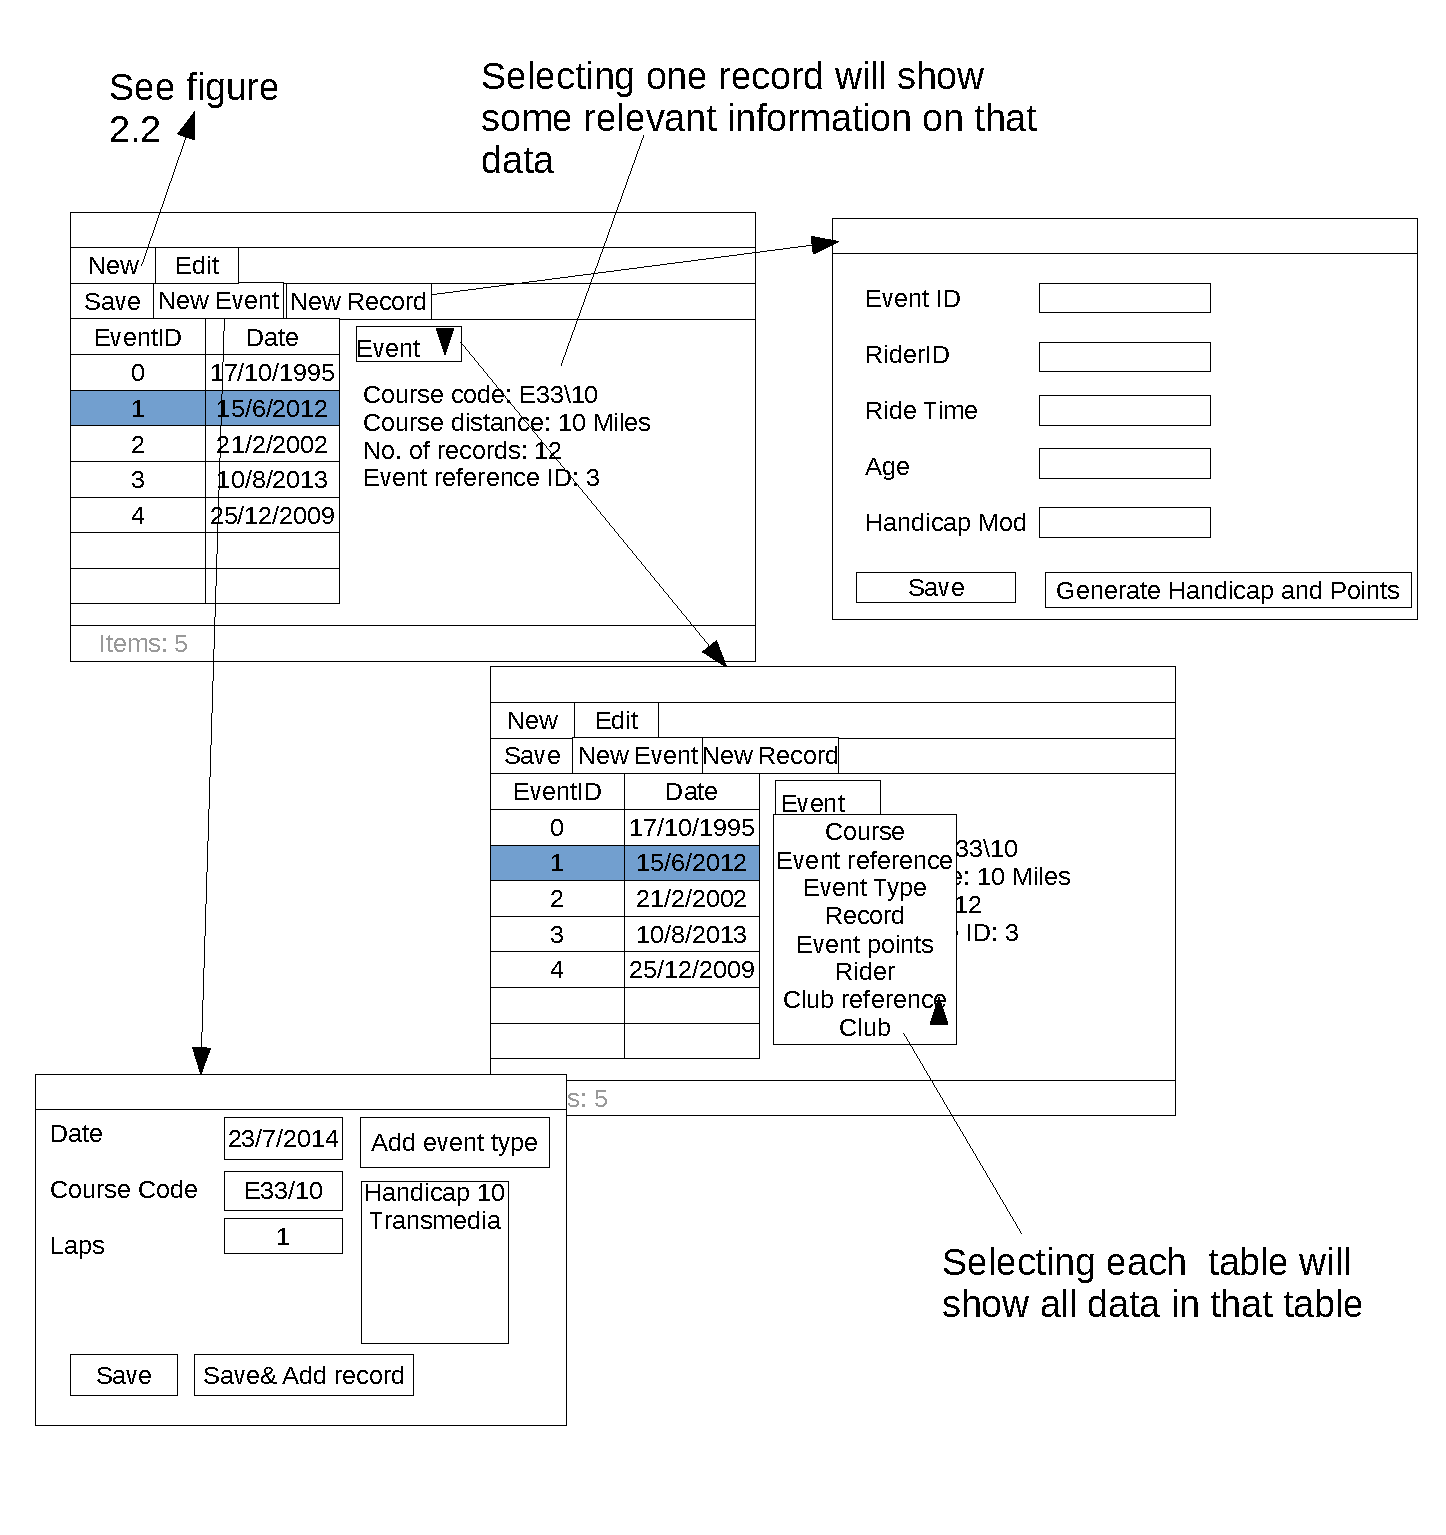
\includegraphics[width=\textwidth]{./UIDesign/BaseMainDrop.pdf}
	\caption{The main layout of the program} \label{fig:The main layout of the program} 	
\end{figure}

\begin{figure}[H]
	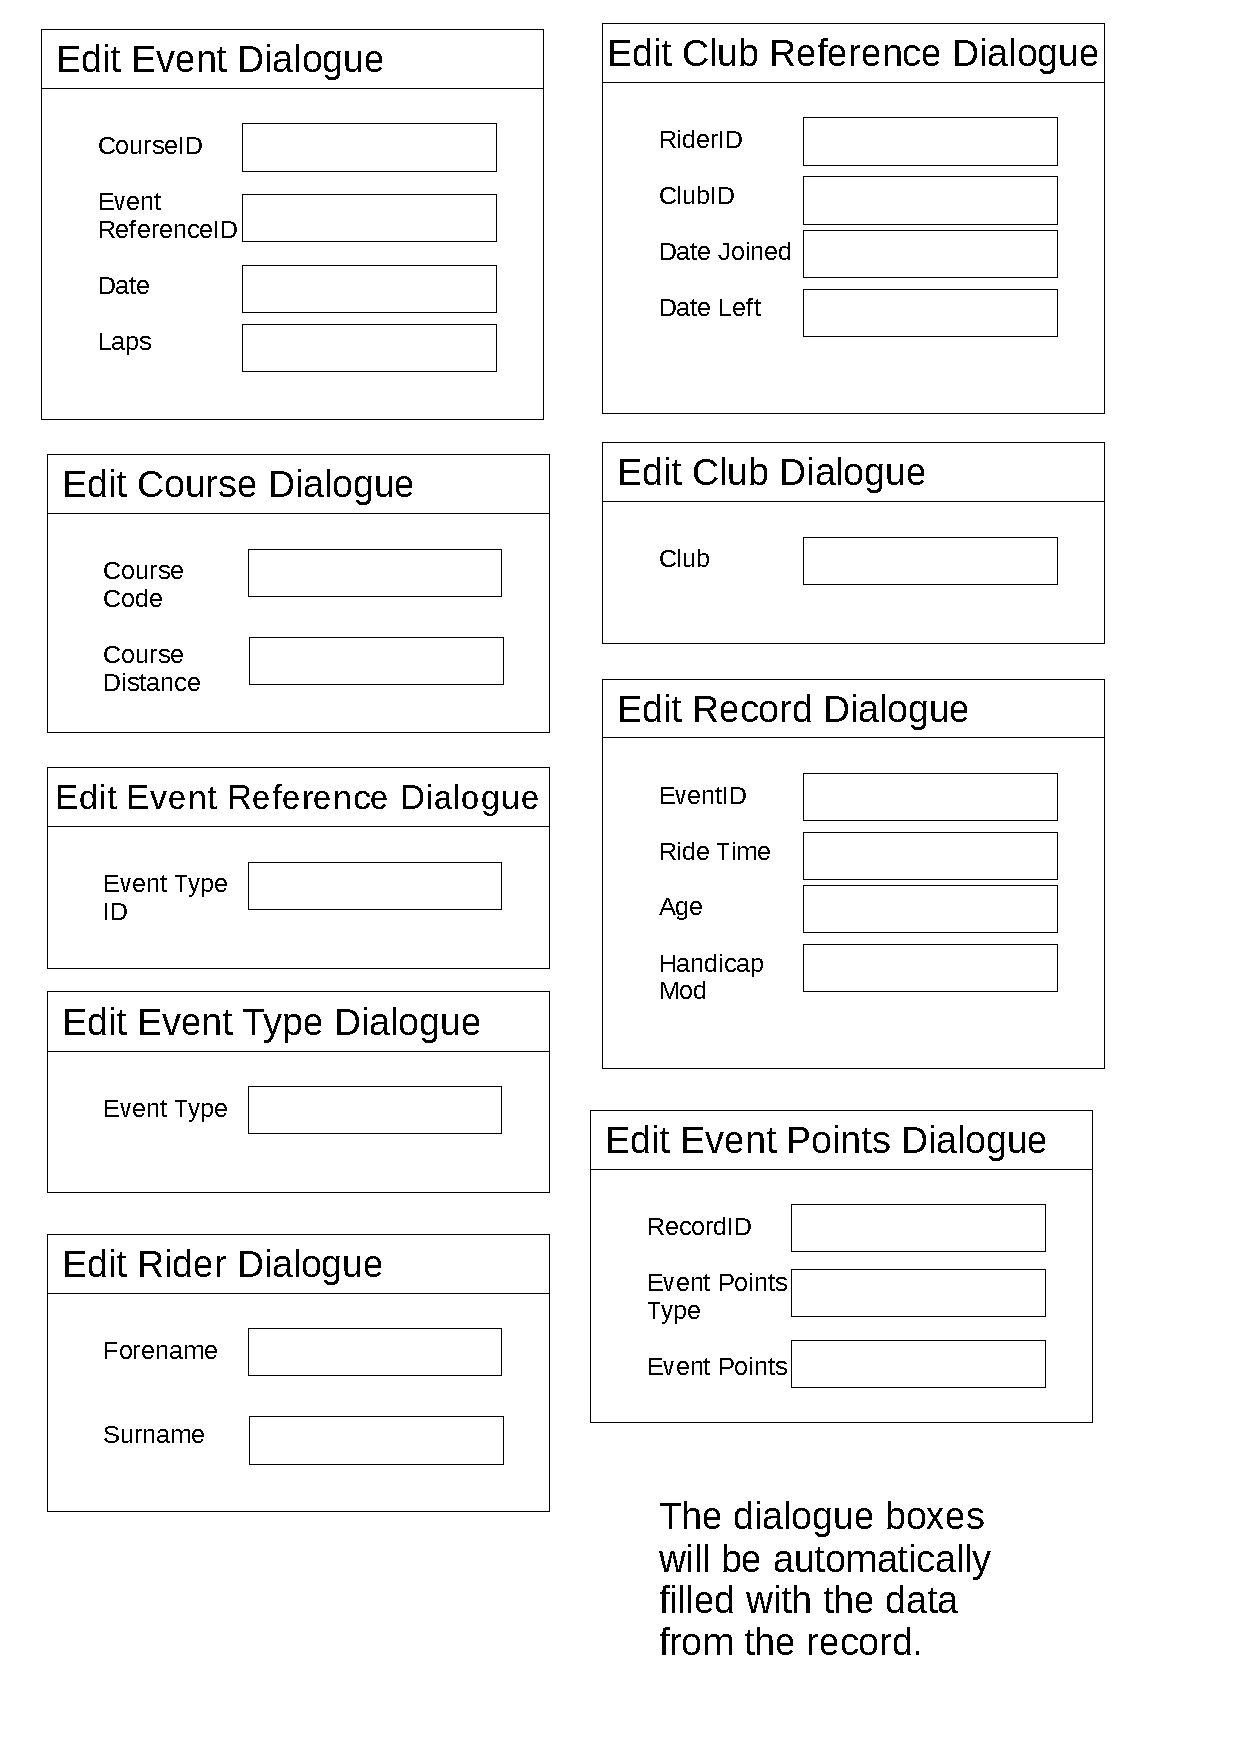
\includegraphics[width=\textwidth]{./UIDesign/EditDialogs.pdf}
	\caption{The dialogue boxes for the edit functions} \label{fig:The dialogue boxes for the edit functions} 	
\end{figure}


\begin{figure}[H]
	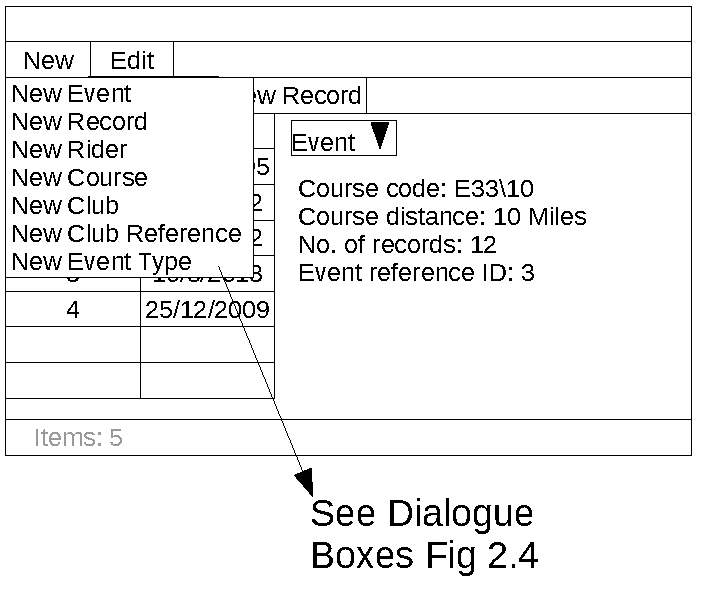
\includegraphics[width=\textwidth]{./UIDesign/DatebaseMainNewDrop.pdf}
	\caption{The new menubar menu} \label{fig:The new menubar menu} 	
\end{figure}

\begin{figure}[H]
	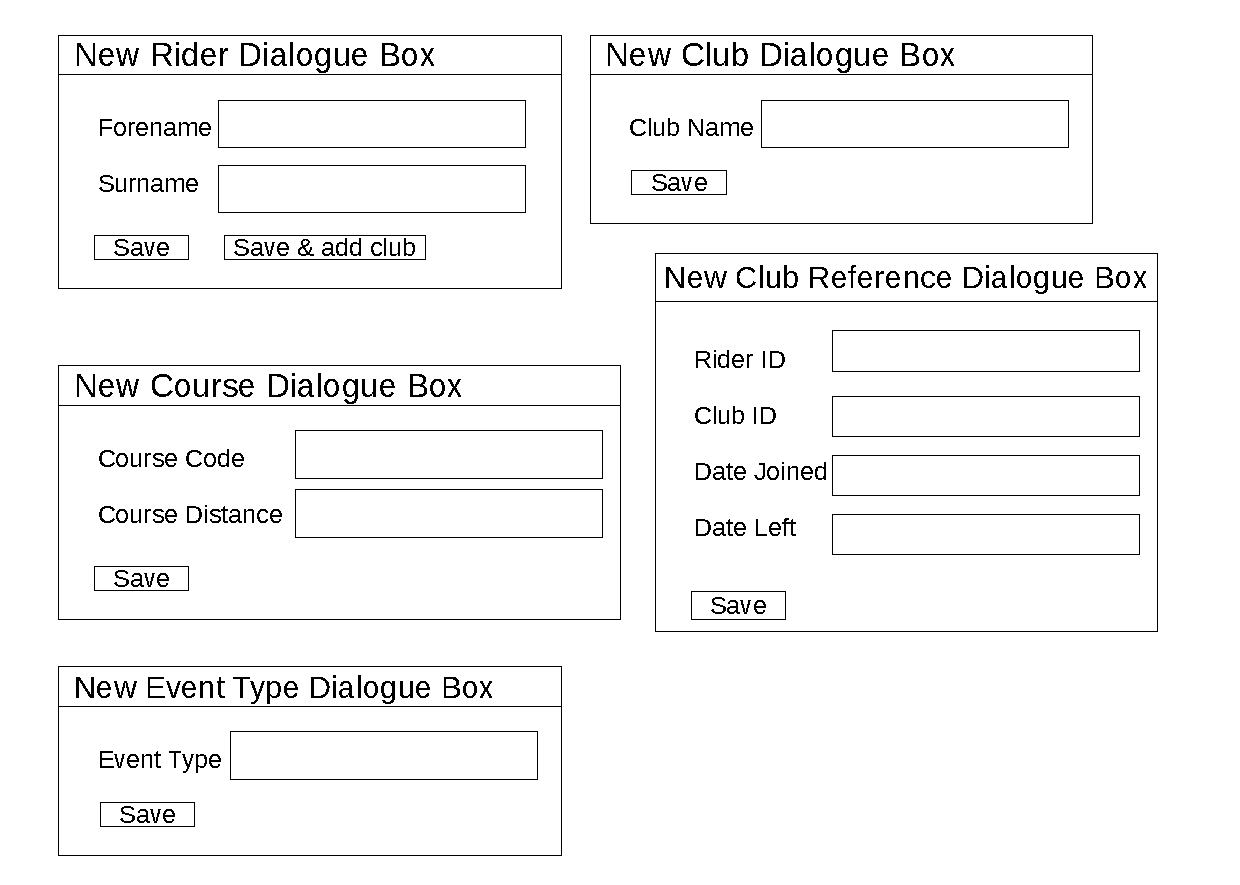
\includegraphics[width=\textwidth]{./UIDesign/Dialogs.pdf}
	\caption{The dialogue boxes for new data} \label{fig:The dialogue boxes for new data} 	
\end{figure}

\subsection{System flowcharts showing an overview of the complete system}

\begin{figure}[H]
	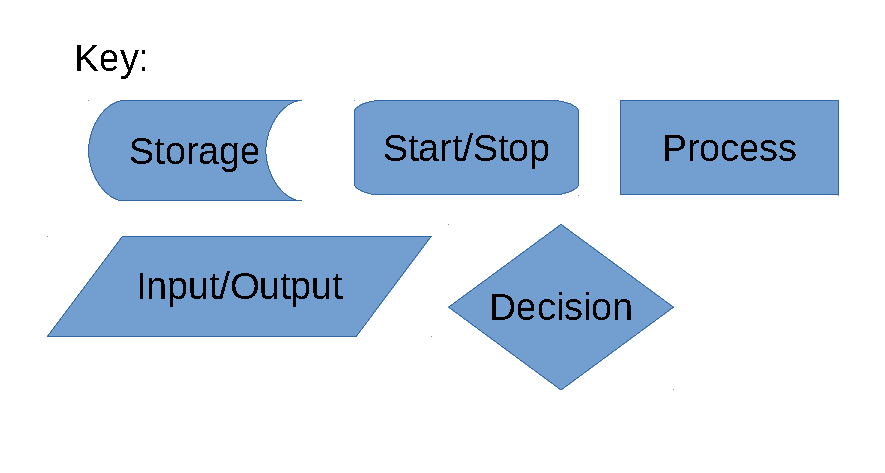
\includegraphics[width=\textwidth]{./FlowChart/Key.pdf}
	\caption{Key for the flow charts} \label{fig:Key for the flow charts} 	
\end{figure}

\begin{figure}[H]
	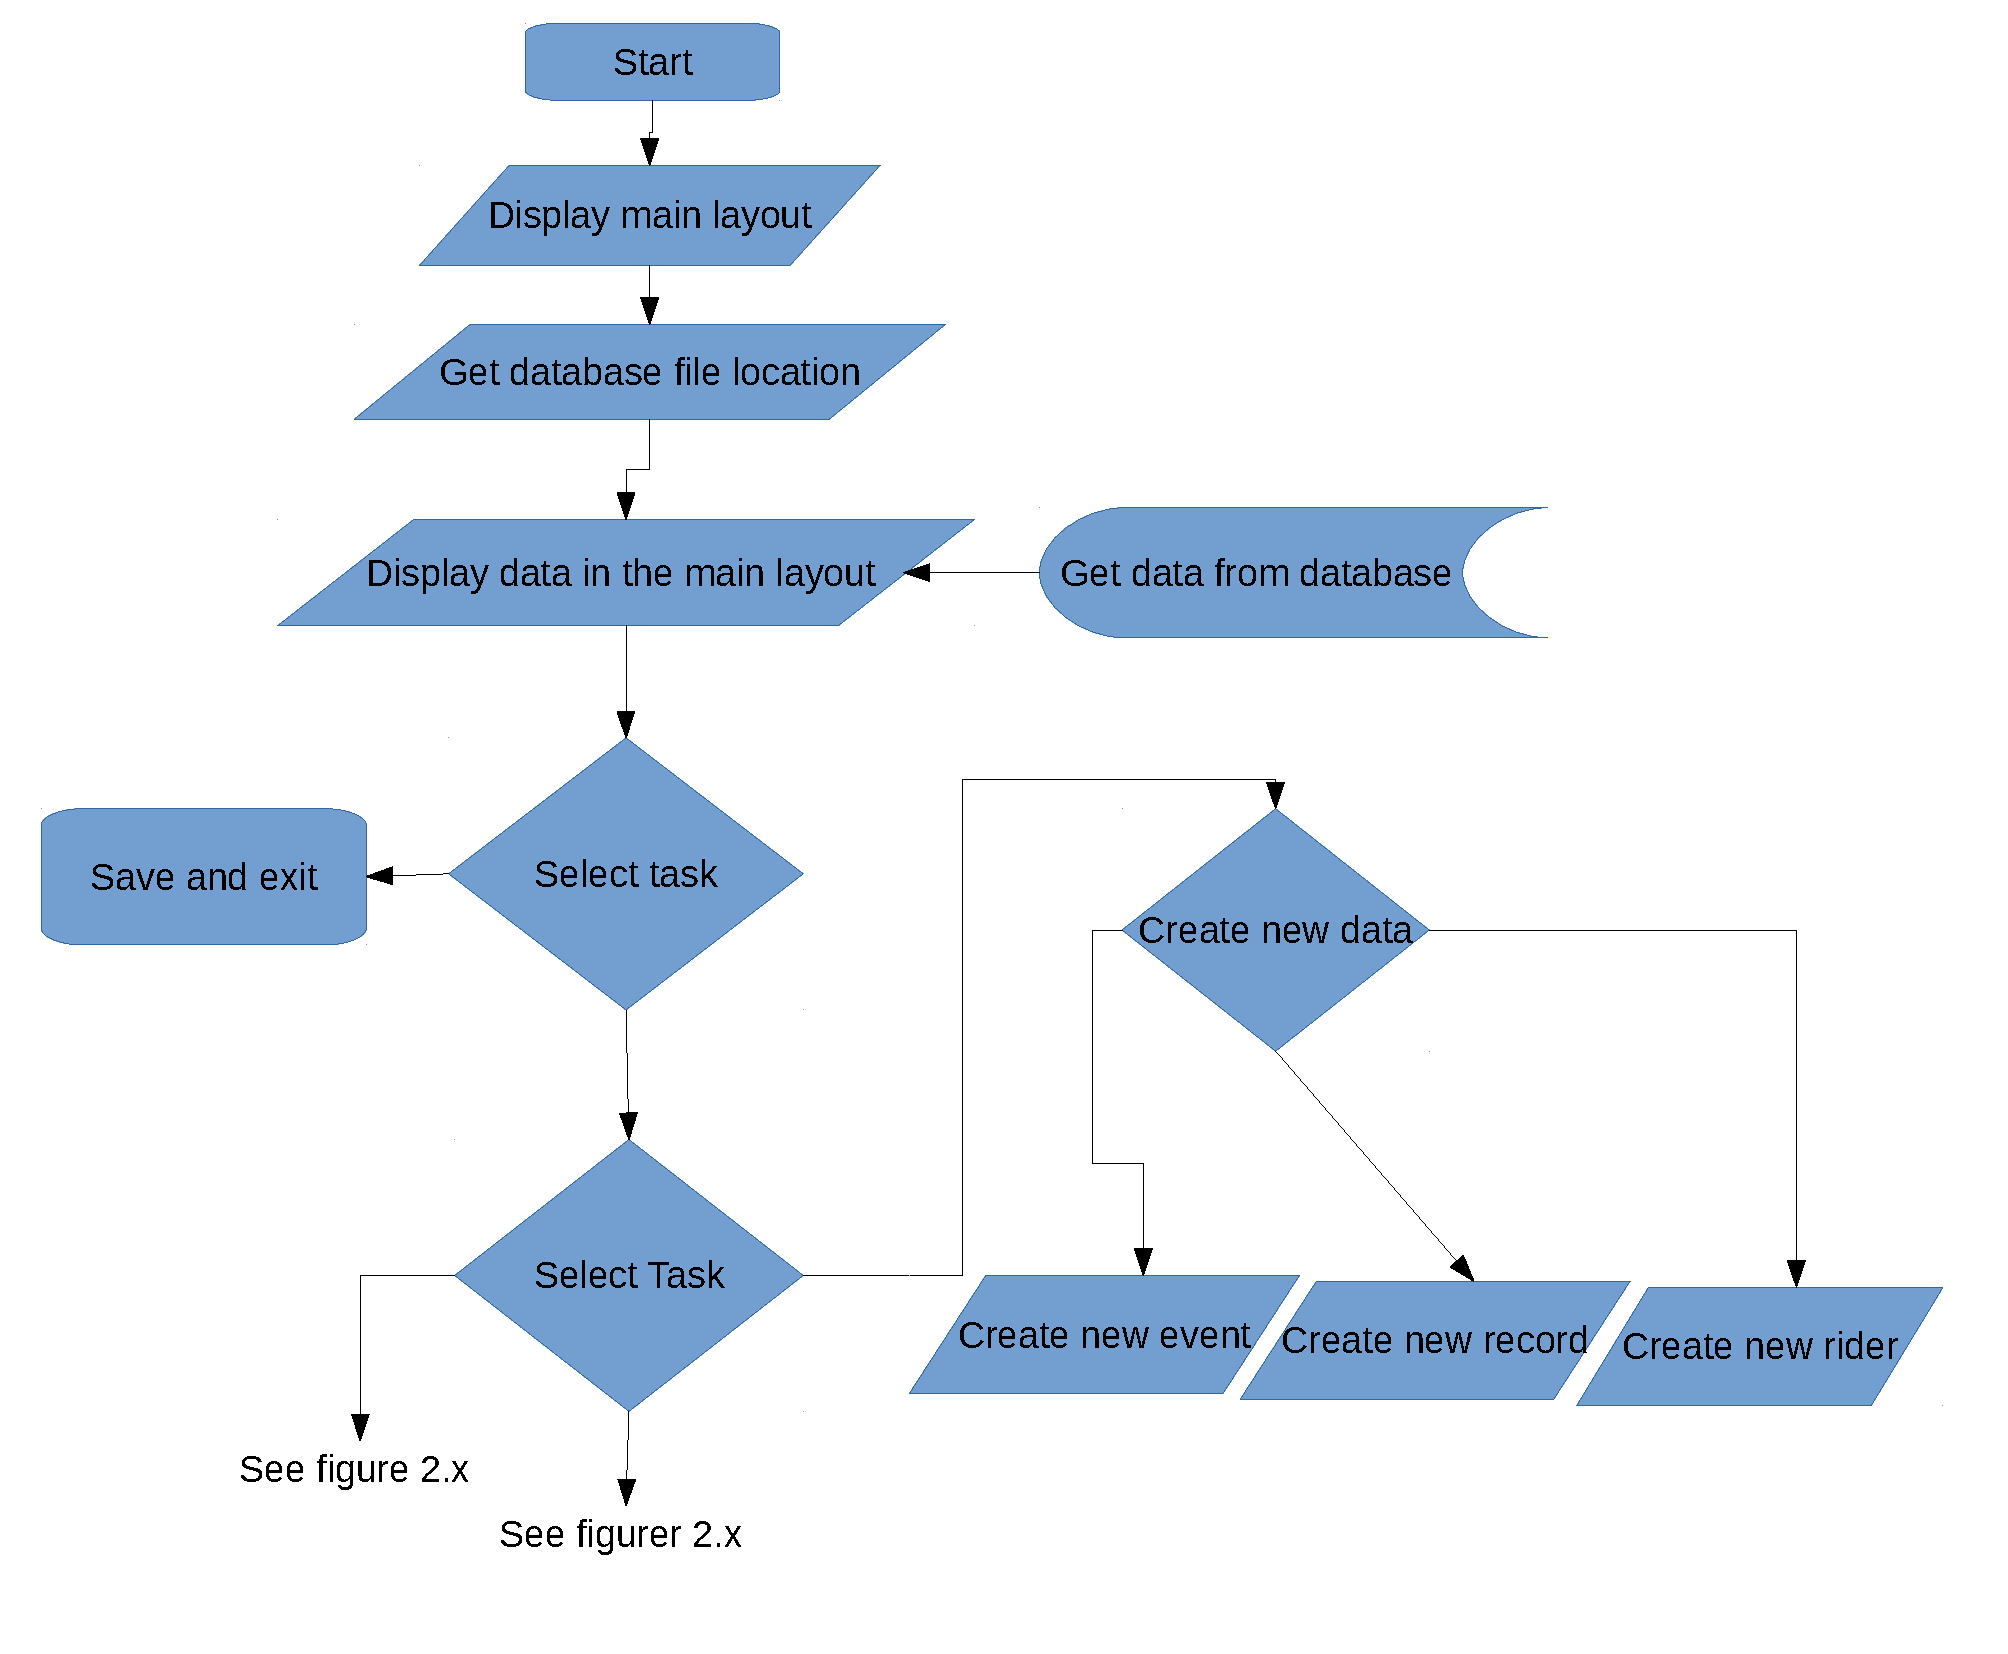
\includegraphics[width=\textwidth]{./FlowChart/SectionOne.pdf}
	\caption{} \label{fig:} 	
\end{figure}

\begin{figure}[H]
	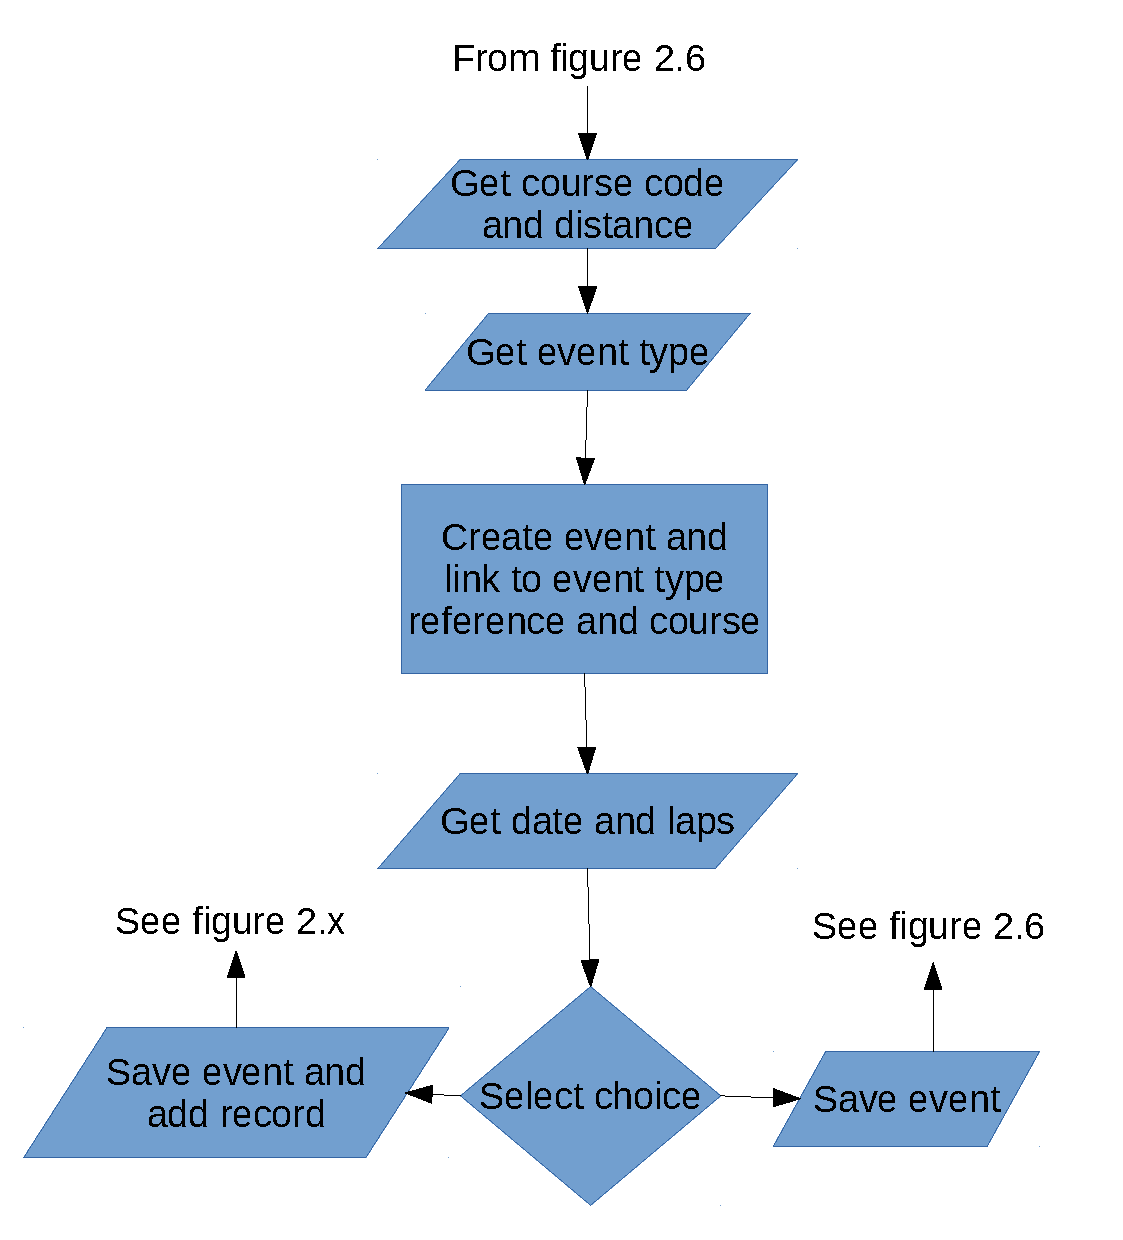
\includegraphics[width=\textwidth]{./FlowChart/SectionTwo.pdf}
	\caption{} \label{fig:} 	
\end{figure}

\begin{figure}[H]
	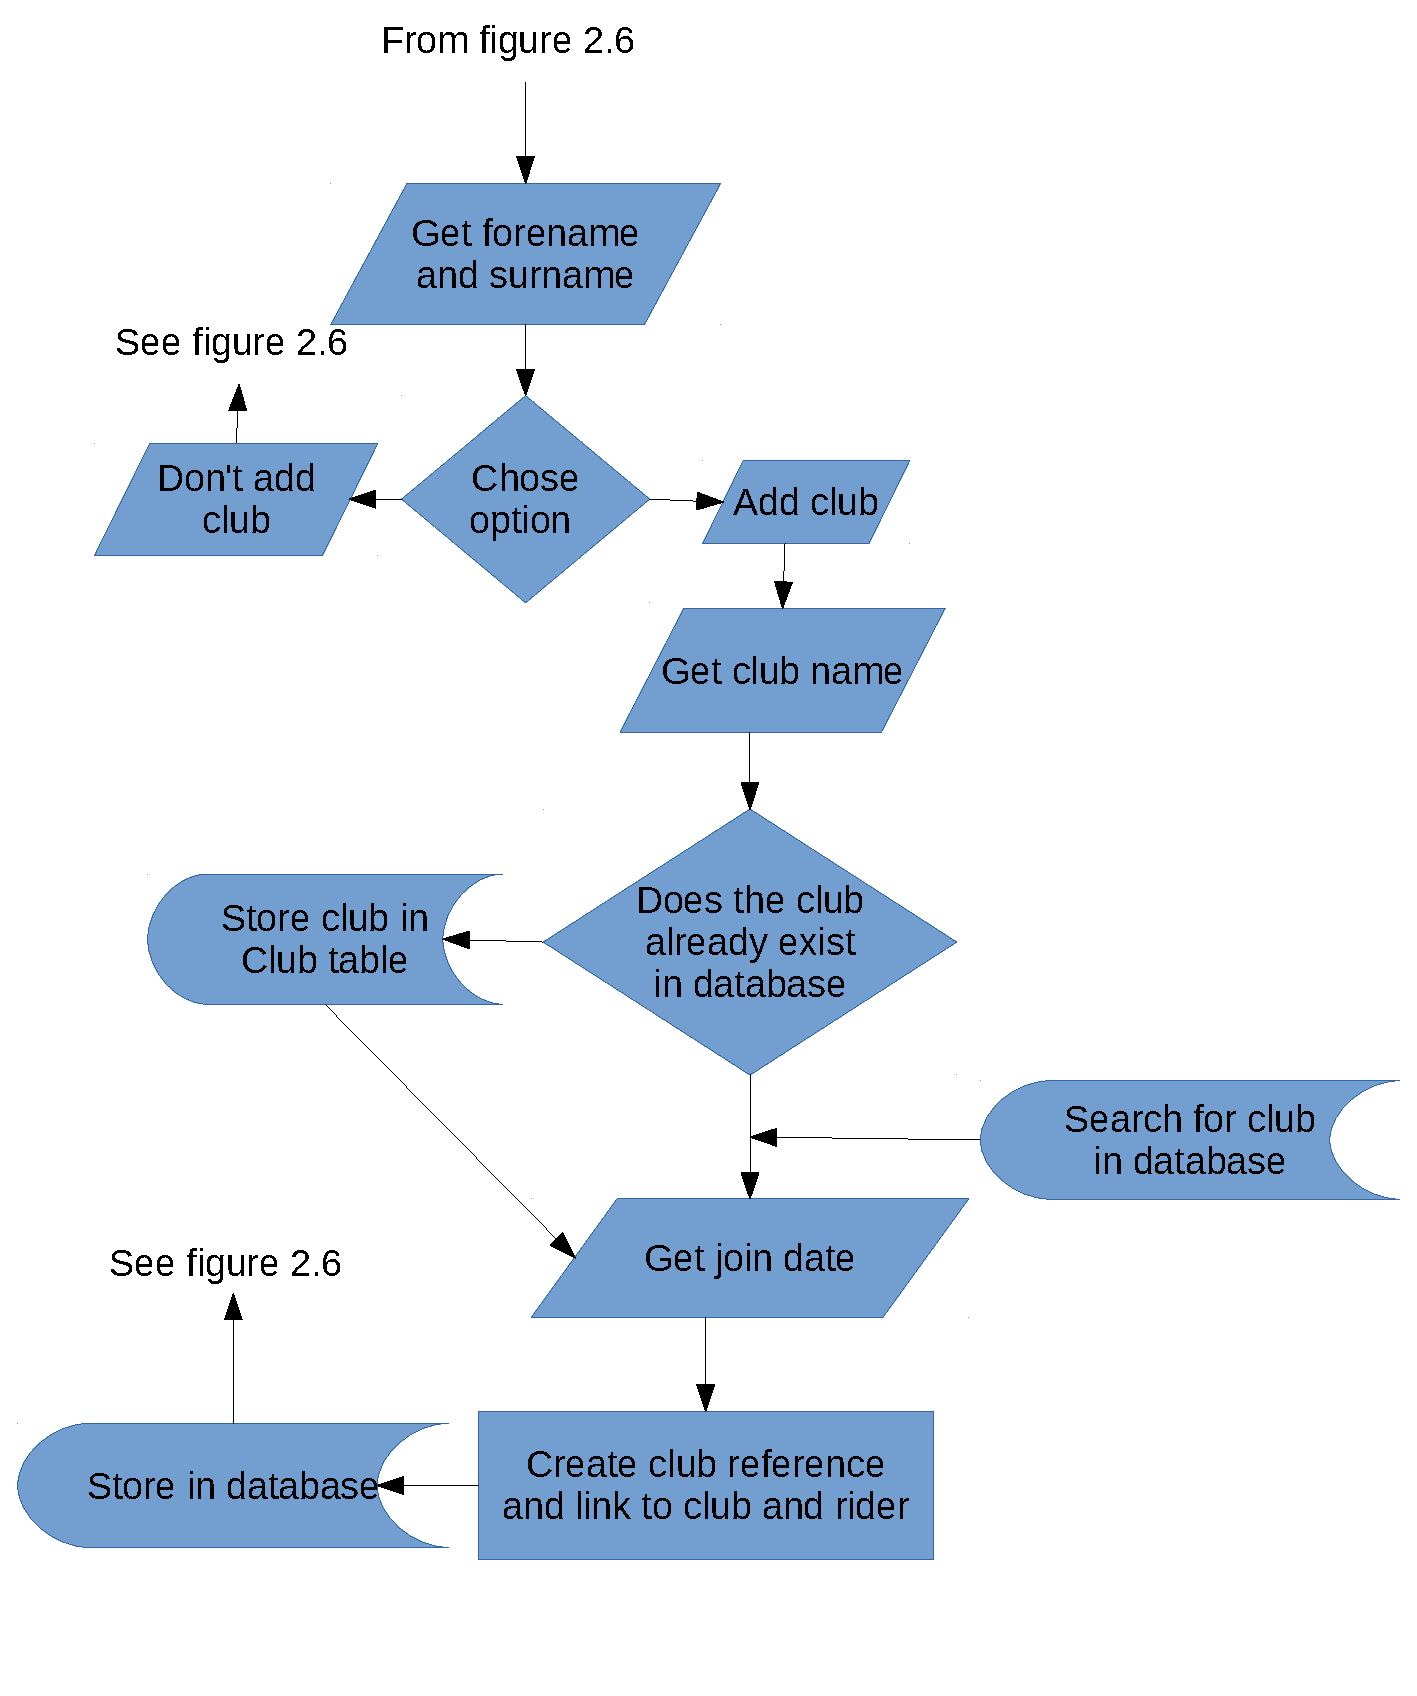
\includegraphics[width=\textwidth]{./FlowChart/SectionThree.pdf}
	\caption{} \label{fig:} 	
\end{figure}

\begin{figure}[H]
	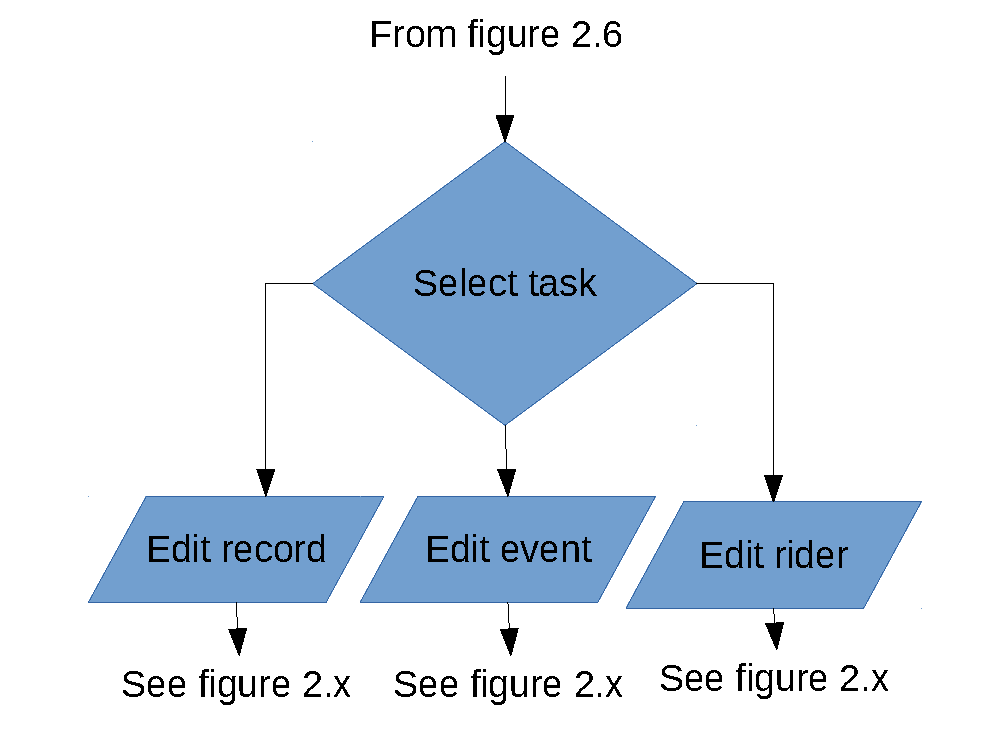
\includegraphics[width=\textwidth]{./FlowChart/SectionFour.pdf}
	\caption{} \label{fig:} 	
\end{figure}

\begin{figure}[H]
	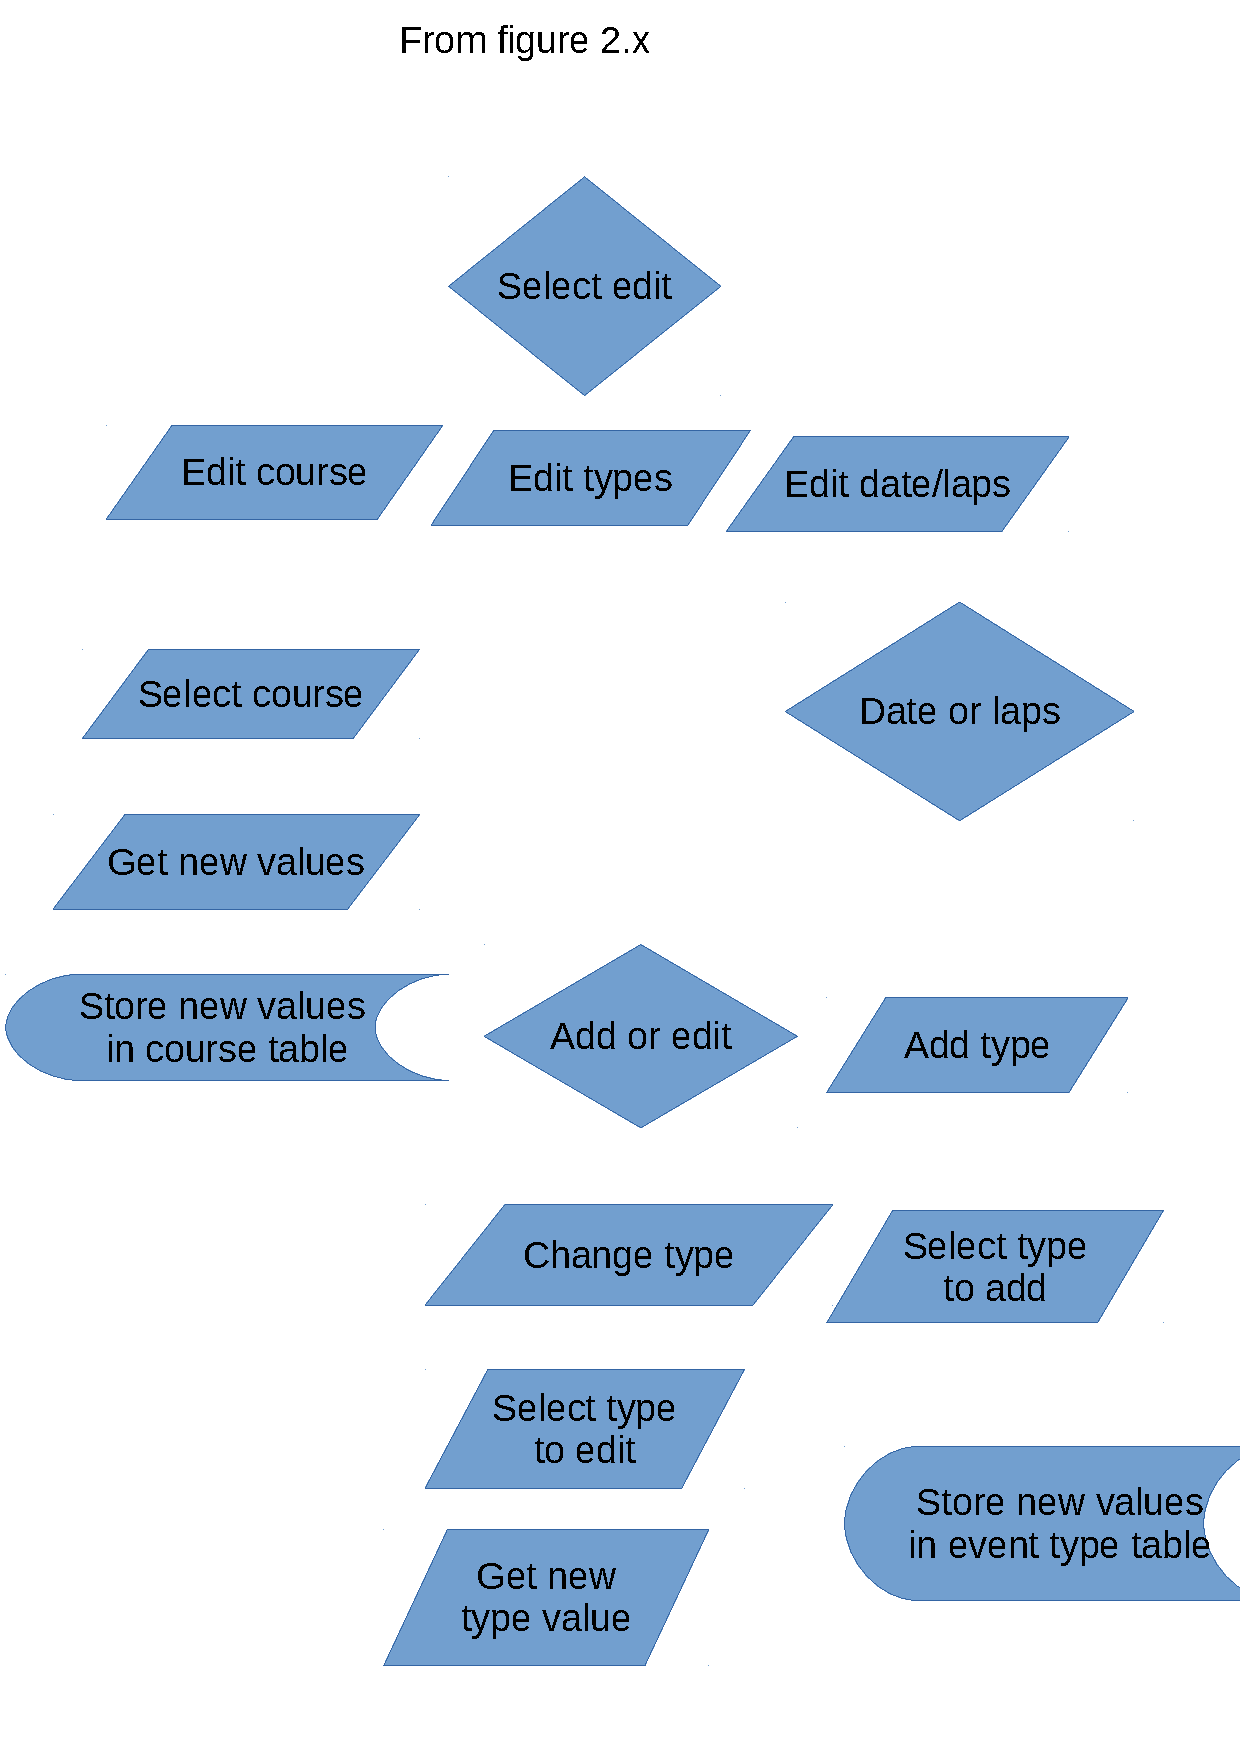
\includegraphics[width=\textwidth]{./FlowChart/SectionFive.pdf}
	\caption{} \label{fig:} 	
\end{figure}

\begin{figure}[H]
	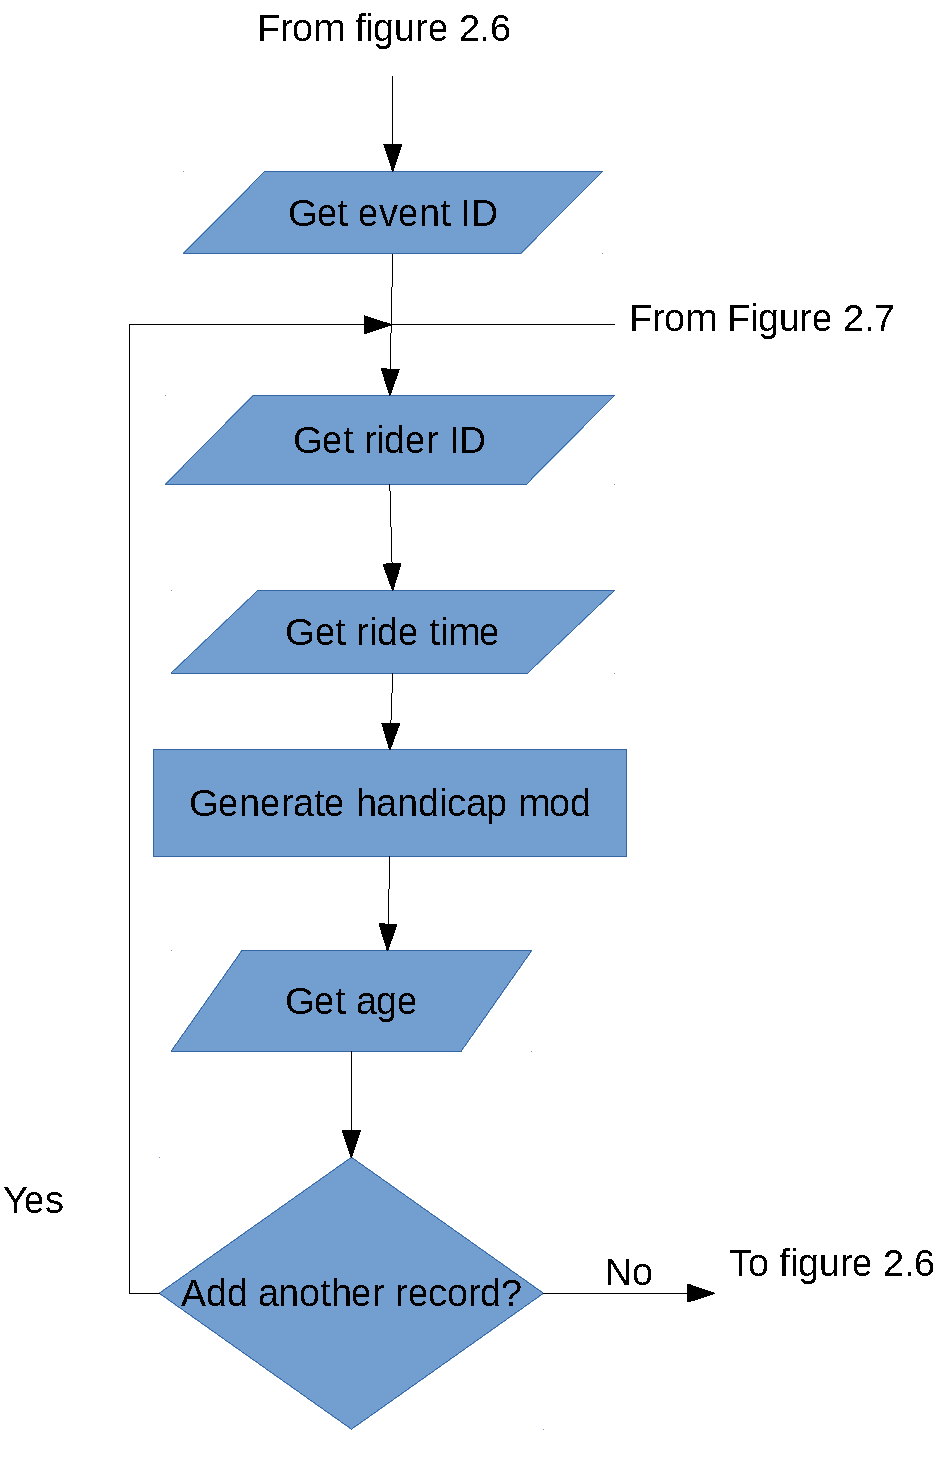
\includegraphics[width=\textwidth]{./FlowChart/SectionSix.pdf}
	\caption{} \label{fig:} 	
\end{figure}

\section{Hardware Spesifiacation}

The hardware spesifiacation of the program will be as follows,

\begin{tabular}{ll}
CPU & Intel Pentium T3400 @ 2.17 GHz\\
RAM & 4 GB DDR2 \\
Storage & 298 GB HDD \\
\end{tabular}

These system spesifiacation have been chosen as my client has this hardware available and would prefer not to have to purchase additional hardware.

\section{Program Structure}

\subsection{Top-down design structure charts}

\subsection{Algorithms in pseudo-code for each data transformation process}

\subsection{Object Diagrams}

\subsection{Class Definitions}

\section{Prototyping}
I decided  to test PyQt to build by understanding of the principles behind programming a UI in python. I created a main window with radio buttons and a push button.

\begin{figure}[H]
    \pythonfile{./Protoyping/MainWindow.py}
    \caption{The code for the main window of the UI test} \label{fig:The code for the main window of the UI test}
\end{figure}

\begin{figure}[H]
    \pythonfile{./Protoyping/RadioButtonWidget.py}
    \caption{The code for the radio button widget of the UI test} \label{fig:The code for the radio button widget of the UI test}
\end{figure}

\section{Definition of Data Requirements}

\subsection{Identification of all data input items}
Here is a list of all the the data input items, all data input will be entered by the user.

\begin{itemize}
\item Age
\item Date
\item Event Type
\item Event Points Type
\item Forename
\item Surname
\item Club
\item Ride Time
\item Course Code
\item Course Distance
\item Date Joined
\item Date Left
\item Laps
\end{itemize}

\subsection{Identification of all data output items}
Here is a list of all the data output item, all data output items will be generated by the system.

\begin{itemize}
\item EventID
\item Event Points
\item RiderID
\item Handicap Mod
\item Event PointsID
\item RecordID
\item CourseID
\item Event ReferenceID
\item Event TypeID
\item ClubID
\item Club ReferenceID
\end{itemize}

\subsection{Explanation of how data output items are generated}

\begin{tabular}{l | p{10cm}}
Data Output & Generation \\ \hline
EventID & Generated when data is added to the event table of the database. \\
Event Points & Event points will be Generated when a event is finished add riders, then all the types of points can be Generated and will be stored in the database. \\
RiderID & Generated when data is added to the rider table of the database.\\
Handicap Mod & Generated when a record has a RiderID and EventID associated with it. Then it will find the quickies time of the same distance and calculated the handicap mod using an algorithm.  \\
Event PointsID & Generated when data is added to the event points table of the database. \\
RecordID & Generated when data is added to the record table of the database. \\
CourseID & Generated when data is added to the course table of the database.\\
Event ReferenceID & Generated when data is added to the event reference table of the database.\\
Event TypeID & Generated when data is added to the event type table of the database. \\
ClubID & Generated when data is added to the club table of the database. \\
Club ReferenceID & Generated when data is added to the club reference table of the database. \\
\end{tabular}

\subsection{Data Dictionary}

\begin{tabular}{|p{1.5cm}|p{1.5cm}|p{1.8cm}|p{2.1cm}|l|p{2.5cm}|}
	\hline
	NAME & DATA TYPE & LENGTH & VALIDATION & EXAMPLE DATA & APPROXIMATE SIZE \\ \hline
	EventID & Integer & 1 - 9999 & Range & 12 & 4 Bytes \\ \hline
	Age & Integer & 10 - 99  & Range & 19 & 4 Bytes \\ \hline
	Date & Sting & 10 Charters & Length and Formatting & 23/12/2014 & 10 Bytes \\ \hline
	Event Points & Integer & 0 - 20 & Range & 15 & 4 Bytes \\ \hline
	EventType & Sting & Up To 10 Charters & Length & Handicap10 & 10 Bytes \\ \hline
	Event PointType & Sting & Up To 25 Charters & Length & 10 Series & 25 Bytes \\ \hline
	Club ReferanceID & Integer & 1 -9999 & Range & 12 & 4 Bytes \\ \hline
	RiderID & Integer & 1 -9999 & Range & 120 & 4 Bytes \\ \hline
	Forename & Sting & Up To 25 Charters & Length & Peter & 25 Bytes \\ \hline
	Surname & Sting & Up To 25 Charters & Length & Millard & 25 Bytes \\ \hline
	Handicap Mod & Sting & 8 Charters & Length and Formatting & 00:01:15 & 8 Bytes \\ \hline
	Event PointsID & Integer & 1 - 9999 & Range & 12 & 4 Bytes \\ \hline
	Club & Sting & Up To 50 Charters & Length & Team Cambridge & 50 Bytes \\ \hline
	RecordID & Integer & 1 - 9999 & Range & 50: & 4 Bytes \\ \hline
	RideTime & Sting & 8 Charters & Length and Formatting & 00:25:26 & 8 Bytes \\ \hline
	CourceID & Integer & 1 - 9999 & Range & 34 & 4 Bytes \\ \hline
	Cource Code & Sting & Up To 10 Charters & Length & F210/CAX & 10 Bytes \\ \hline
	Cource Distance & Integer & 1 - 999 & Range & 25 & 4 Bytes \\ \hline
	Date Joined & Sting & 10 Charters & Length and Formatting & 12/12/2015 & 10 Bytes \\ \hline
	DateLeft & Sting & 10 Charters & Length and Formatting & 24/10/1995 & 10 Bytes \\ \hline
	Event ReferanceID & Integer & 1 - 9999 & Range & 230 & 4 Bytes \\ \hline
	Event TypeID & Integer & 1 - 9999 & Range & 666 & 4 Bytes \\ \hline
	ClubID & Integer & 1 - 9999 & Range & 624 & 4 Bytes \\ \hline
	Laps & Integer & 1 - 99 & Range & 2 & 4 Bytes \\ \hline
\end{tabular}
\subsection{Identification of appropriate storage media}

\section{Database Design}

\subsection{Normalisation}

\subsubsection{ER Diagrams}
\begin{figure}[H]
    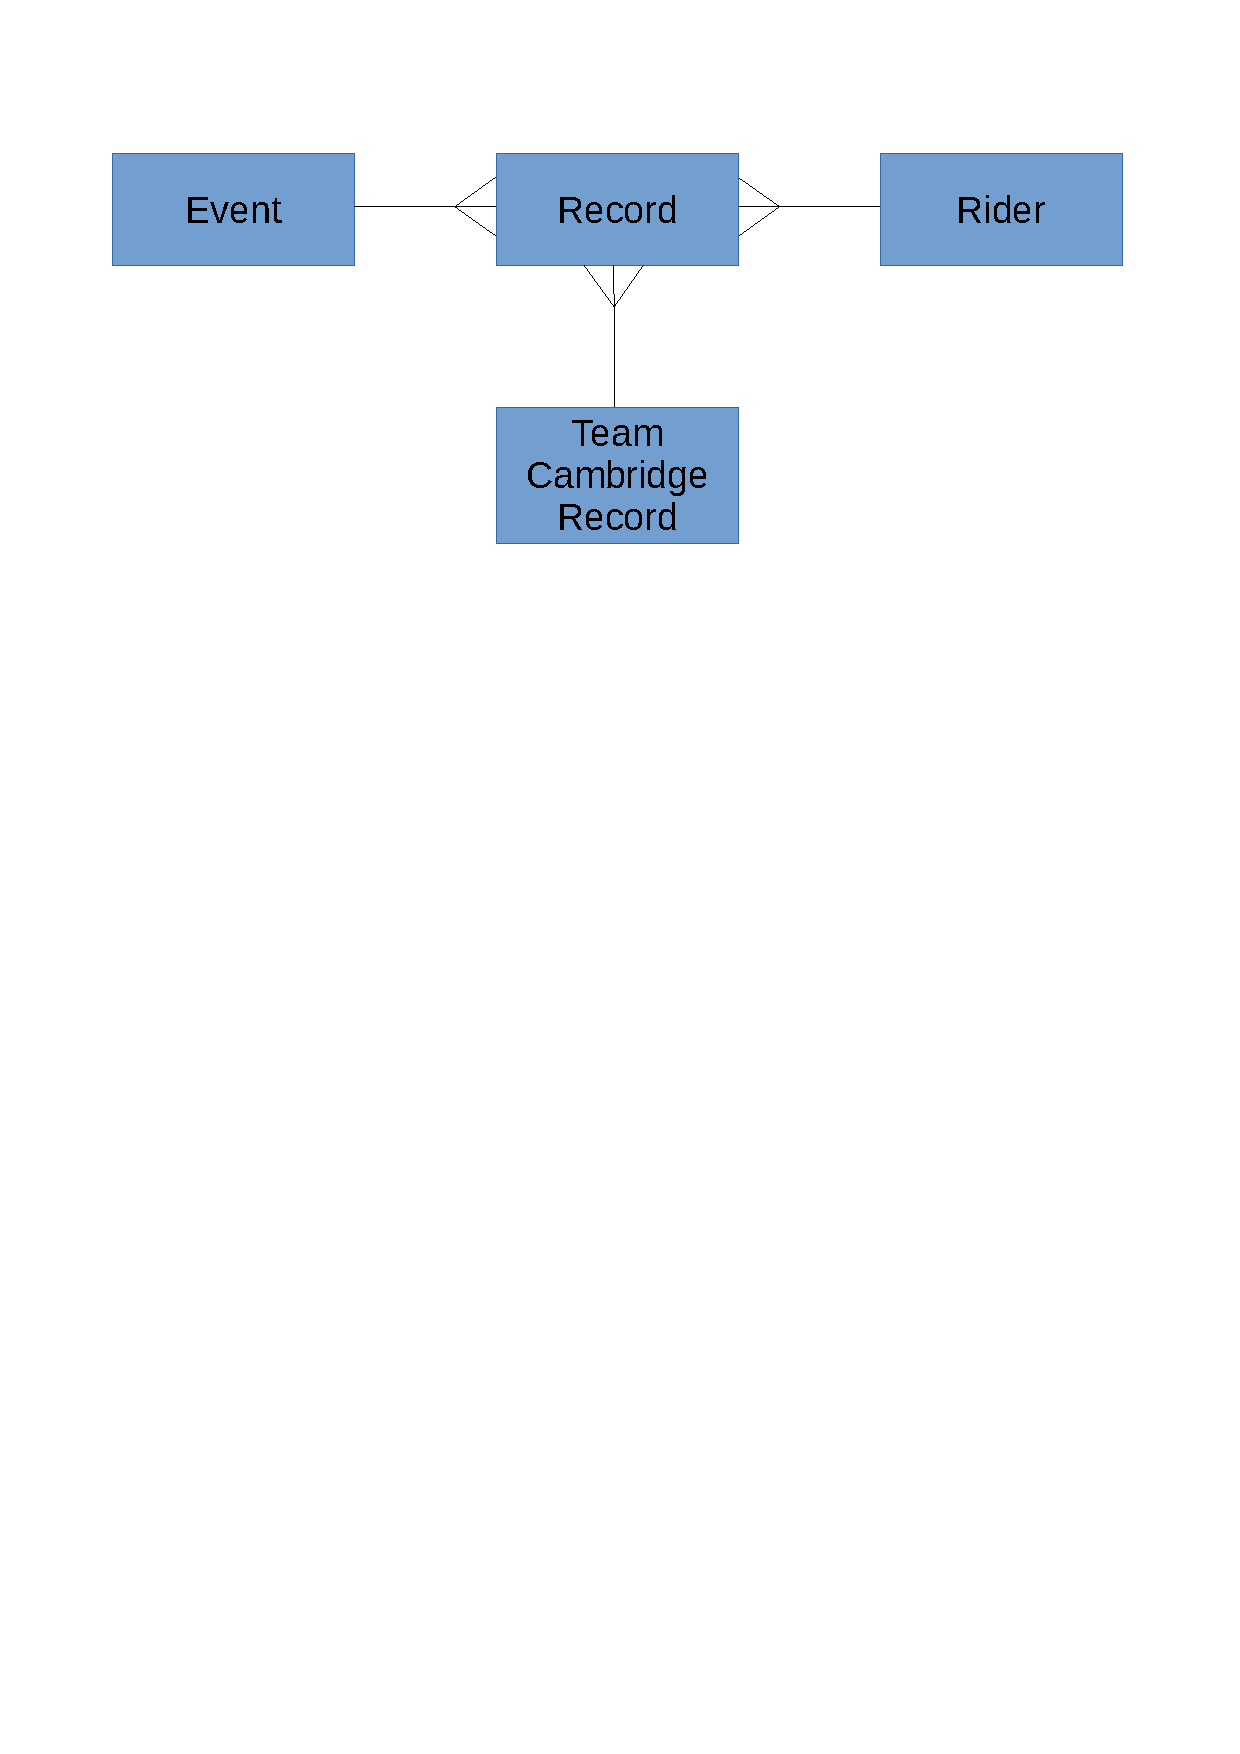
\includegraphics[width=\textwidth]{./ER/ERDesing.pdf}
\end{figure}

\subsubsection{Entity Descriptions}

Event(\underline{EventID}, \emph{CourseID} , \emph{EventReferanceID}, Date, Laps )

Course(\underline{CourseID}, CourseCode, CourseDistance)

Event Referance(\underline{EventReferanceID}, \emph{EventTypeID})

Event Type(\underline{EventTypeID}, EventType)

Rider(\underline{RiderID}, Forename, Surname)

Club Reference(\underline{ClubReferance}, \emph{RiderID}, \emph{ClubID}, DateJoined, DateLeft)

Club(\underline{ClubID}, Club)

Record(\underline{RecordID}, \emph{EventID}, RideTime, Age, HandicapMod)

Event Points(\underline{EventPointsID}, \emph{RecordID}, EventPointsType, EventPoints)

\subsubsection{UNF to 3NF}
\underline{UNF}


\begin{tabular}{l l l}
EventID        & Age              & Date               \\
EventPoints    & EventType        & EventPointType     \\
ClubReferance  & RiderID          & Forename           \\
Surname        & HandicapMod      & EventPointsID      \\
Club           & RecordID         & RideTime           \\
CourceID       & CourceCode       & CourceDistance     \\
DateJoined     & DateLeft         & EventReferanceID   \\
EventTypeID    & ClubID           & Laps               \\

\end{tabular}

\underline{1NF}

\begin{tabular}{|l l|l|}
\hline
REPEATING           &                 & NON-REPEATING       \\ \hline
\underline{RecordID}& RideTime        & \underline{EventID} \\ \hline
\underline{EventID} & EventPointsType & Date                \\ \hline
ClubReferance       & DateLeft        & CourseID            \\ \hline
Surname             & HandicapMod     & CourseCode          \\ \hline
DateJoined          & RiderID         & CorseDistance       \\ \hline 
EventPointsID       & Age             & EventReferanceID    \\ \hline
EventTypeID         & ClubID          & Laps                \\ \hline
\end{tabular}




\underline{2NF}

\begin{tabular}{|l|l|}
\hline
\underline{RecordID} & \underline{EventID} \\ \hline
Forename             & Date                \\ \hline
Surname              & CourceID            \\ \hline
ClubReferance        & CourceCode          \\ \hline
Club                 & CourceDistance      \\ \hline
DateJoined           & EventTypeID         \\ \hline
DateLeft             & EventType           \\ \hline
ClubID               & EventReferanceID    \\ \hline
                     & Laps                \\ \hline
\underline{RecordID} &                     \\ \hline
\underline{EventID}  &                     \\ \hline 
EventPointsID        &                     \\ \hline
RideTIme             &                     \\ \hline
Age                  &                     \\ \hline
HandicapMod          &                     \\ \hline
EventPoints          &                     \\ \hline
EventPointsType      &                     \\ \hline
\end{tabular}

\underline{3NF}

\begin{tabular}{|l|l|l|l|}
\hline
\begin{tabular}{l}
	\\
	\underline{EventID}     \\
	\emph{CourseID}         \\
	\emph{EventReferanceID} \\
	Date                    \\
	Laps                    \\
	\\
\end{tabular}& \begin{tabular}{l}
	\underline{CourseID} \\
	CourseCode           \\
	CourseDistance       \\
\end{tabular} & \begin{tabular}{l}
	\underline{EventReferanceID} \\
	\emph{EventTypeID}           \\
\end{tabular} &\begin{tabular}{l}
	\underline{RiderID} \\
	Forename            \\
	Surname             \\
\end{tabular} \\ \hline
\begin{tabular}{l}
	\underline{ClubReference} \\
	\emph{RiderID}            \\
	\emph{ClubID}             \\
	DateJoined                \\
	DateLeft                  \\
\end{tabular} & \begin{tabular}{l}
	\\
	\underline{RecordID} \\
	\emph{EventID}       \\
	\emph{RiderID }      \\
	RideTime             \\
	Age                  \\
	HandicapMod          \\
	\\
\end{tabular} & \begin{tabular}{l}
	\underline{EventPointsID} \\
	\emph{RecordID}           \\
	EventPointsType           \\
	EventPoints               \\
\end{tabular} & \begin{tabular}{l}
	\underline{ClubID} \\
	Club               \\
\end{tabular} \\ \hline
\begin{tabular}{l}
	\\
	\underline{EventTypeID} \\
	EventType               \\
	\\
\end{tabular} & & & \\ \hline 
\end{tabular}

\section{Security and Integrity of the System and Data}

\subsection{Security and Integrity of Data}
My system will not fall under the data protection act as no personal data is being stored. This mean that I will not have to use encryption on the database nor will I have to ensure data is kept up to date and accurate.
\subsection{System Security}
As my system will not have to comply with the data protection act I will not be implementing any system security.
\section{Validation}

\section{Testing}

\begin{landscape}
\subsection{Outline Plan}

\begin{center}
    \begin{tabular}{|p{2cm}|p{5cm}|p{5cm}|p{4cm}|}
        \hline
        \textbf{Test Series} & \textbf{Purpose of Test Series} & \textbf{Testing Strategy} & \textbf{Strategy Rationale}\\ \hline
        1 & Test the flow of control of the user interface  & Top-Down testing &  \\ \hline
        2 & Validation of user input & Bottom-Up testing &  \\ \hline
        3 & Validation of system output & System Testing & \\ \hline
        4 & Validation of core system functionality & White box testing & \\ \hline
        5 & System performs as required by the specification & Black box testing & \\ \hline
    \end{tabular}
\end{center}

\subsection{Detailed Plan}

\begin{center}
    \begin{longtable}{|p{1.5cm}|p{2.5cm}|p{2.5cm}|p{2cm}|p{2cm}|p{2cm}|p{2cm}|p{2cm}|}
        \hline
        \textbf{Test Series} & \textbf{Purpose of Test} & \textbf{Test Description} & \textbf{Test Data} & \textbf{Test Data Type (Normal/ Erroneous/ Boundary)} & \textbf{Expected Result} & \textbf{Actual Result} & \textbf{Evidence}\\ \hline
        1.01 & Test the file dialogue box & This should out put a file location and link ot the main screen & double click on file location & Normal & the database should be loaded up on the main screen &  &  \\ \hline
        
        1.02 & Test the change table buttons in the menu bar  & This should change the main layout so that it shows the table of the selected type & Click on each button in the table section of the menu bar & Normal & the main layout changes to the table of the selected type & & \\ \hline
        
        1.03 & Test the add data button for the rider table & Click on the add data button while in the club reference table & click on the add data button while in the rider table & normal & display the add data dialogue box for the rider table & & \\ \hline
        1.04 & Test the add data button for the club reference table & Click on the add data button while in the club table & click on the add data button while in the club reference table & normal & display the add data dialogue box for the club reference table & & \\ \hline
        1.05 & Test the add data button for the club  table & Click on the add data button while in the rider table & click on the add data button while in the club table & normal & display the add data dialogue box for the club  table & & \\ \hline
        1.06 & Test the add data button for the record  table & Click on the add data button while in the record table & click on the add data button while in the record table & normal & display the add data dialogue box for the record  table & & \\ \hline
        1.07 & Test the add data button for the event points  table & Click on the add data button while in the event points table & click on the add data button while in the event points table & normal & display the add data dialogue box for the event points  table & & \\ \hline
        1.08 & Test the add data button for the event  table & Click on the add data button while in the event table & click on the add data button while in the event table & normal & display the add data dialogue box for the event  table & & \\ \hline
        1.09 & Test the add data button for the course  table & Click on the add data button while in the course table & click on the add data button while in the course table & normal & display the add data dialogue box for the course  table & & \\ \hline
        1.10 & Test the add data button for the event reference  table & Click on the add data button while in the event reference table & click on the add data button while in the event reference table & normal & display the add data dialogue box for the event reference  table & & \\ \hline
        1.11 & Test the add data button for the event type  table & Click on the add data button while in the event type table & click on the add data button while in the event type table & normal & display the add data dialogue box for the event type  table & & \\ \hline
        
        
        1.12 & Test the edit data button for the rider table & Click on the edit data button while in the club reference table & click on the edit data button while in the rider table & normal & display the edit data dialogue box for the rider table & & \\ \hline
        1.13 & Test the edit data button for the club reference table & Click on the edit data button while in the club table & click on the edit data button while in the club reference table & normal & display the edit data dialogue box for the club reference table & & \\ \hline
        1.14 & Test the edit data button for the club  table & Click on the edit data button while in the rider table & click on the edit data button while in the club table & normal & display the edit data dialogue box for the club  table & & \\ \hline
        1.15 & Test the edit data button for the record  table & Click on the edit data button while in the record table & click on the edit data button while in the record table & normal & display the edit data dialogue box for the record  table & & \\ \hline
        1.16 & Test the edit data button for the event points  table & Click on the edit data button while in the event points table & click on the edit data button while in the event points table & normal & display the edit data dialogue box for the event points  table & & \\ \hline
        1.17 & Test the edit data button for the event  table & Click on the edit data button while in the event table & click on the edit data button while in the event table & normal & display the edit data dialogue box for the event  table & & \\ \hline
        1.18 & Test the edit data button for the course  table & Click on the edit data button while in the course table & click on the edit data button while in the course table & normal & display the edit data dialogue box for the course  table & & \\ \hline
        1.19 & Test the edit data button for the event reference  table & Click on the edit data button while in the event reference table & click on the edit data button while in the event reference table & normal & display the edit data dialogue box for the event reference  table & & \\ \hline
        1.20 & Test the edit data button for the event type  table & Click on the edit data button while in the event type table & click on the edit data button while in the event type table & normal & display the edit data dialogue box for the event type  table & & \\ \hline
        
        1.21 & Test the delete data button for the rider table & Click on the delete data button while in the club reference table & click on the delete data button while in the rider table & normal & display the delete data dialogue box for the rider table & & \\ \hline
        1.22 & Test the delete data button for the club reference table & Click on the delete data button while in the club table & click on the delete data button while in the club reference table & normal & display the delete data dialogue box for the club reference table & & \\ \hline
        1.23 & Test the delete data button for the club  table & Click on the delete data button while in the rider table & click on the delete data button while in the club table & normal & display the delete data dialogue box for the club  table & & \\ \hline
        1.24 & Test the delete data button for the record  table & Click on the delete data button while in the record table & click on the delete data button while in the record table & normal & display the delete data dialogue box for the record  table & & \\ \hline
        1.25 & Test the delete data button for the event points  table & Click on the delete data button while in the event points table & click on the delete data button while in the event points table & normal & display the delete data dialogue box for the event points  table & & \\ \hline
        1.26 & Test the delete data button for the event  table & Click on the delete data button while in the event table & click on the delete data button while in the event table & normal & display the delete data dialogue box for the event  table & & \\ \hline
        1.27 & Test the delete data button for the course  table & Click on the delete data button while in the course table & click on the delete data button while in the course table & normal & display the delete data dialogue box for the course  table & & \\ \hline
        1.28 & Test the delete data button for the event reference  table & Click on the delete data button while in the event reference table & click on the delete data button while in the event reference table & normal & display the delete data dialogue box for the event reference  table & & \\ \hline
        1.29 & Test the delete data button for the event type  table & Click on the delete data button while in the event type table & click on the delete data button while in the event type table & normal & display the delete data dialogue box for the event type  table & & \\ \hline
        
        1.30 & Test the line edits of the dialogue box & Testing the line edits used in the dialogue boxes & "Peter" in the forename section of the search data for the rider table & Normal & "Peter" should be held in the line edit and can be returned & & \\ \hline 
    \end{longtable}
\end{center}
\end{landscape}
